\documentclass[letterpaper,10pt,draftclsnofoot,onecolumn]{IEEEtran}

\usepackage{graphicx}                                        
\usepackage{amssymb}                                         
\usepackage{amsmath}                                         
\usepackage{amsthm}                                          
%\usepackage[pdftex]{graphicx}

\usepackage{pdfpages}
\usepackage{array}

\usepackage{alltt}                                           
\usepackage{float}
\usepackage{color}
\usepackage{url}
\usepackage{upquote}
\usepackage{array}
\usepackage{balance}
\usepackage[TABBOTCAP, tight]{subfigure}
\usepackage{enumitem}
\usepackage{pstricks, pst-node}
\usepackage[utf8]{inputenc}

\usepackage{listings}

\usepackage{geometry}
\geometry{textheight=8.5in, textwidth=6in}

%random comment

\newcommand{\cred}[1]{{\color{red}#1}}
\newcommand{\cblue}[1]{{\color{blue}#1}}

\usepackage{hyperref}
\usepackage{geometry}

\def\name{Sinan Topkaya}

%pull in the necessary preamble matter for pygments output
%\input{pygments.tex}

%% The following metadata will show up in the PDF properties
\hypersetup{
  colorlinks = true,
  urlcolor = black,
  pdfauthor = {\name},
  pdfkeywords = {cs444  Final},
  pdftitle = {CS 444 Final: Final},
  pdfsubject = {CS 444},
  pdfpagemode = UseNone
}

\parindent = 0.0 in
\parskip = 0.2 in

\begin{document}


	\begin{titlepage}
		
		\begin{center}
		\bigbreak	
		\textbf{Operating System Feature Comparison}
		\bigbreak
		by Sinan Topkaya
		\smallbreak
		CS 444 - Spring 2016
		\end{center}
		\vfill
		
		Abstract: This paper will examine processes, threads and CPU scheduling, I/O, interrupts and memory management for Windows and FreeBSD operating systems. It will mainly be about how these operating systems implement them and how is it different or similar compared to Linux. This paper also includes the extra credit work.
		
	\end{titlepage}

\section*{Processes, Threads and CPU Scheduling}
A process is a program that is running on your computer. This can be anything from a small background task, such as a spell-checker or system events handler to a full-blown application like Internet Explorer or Microsoft Word. All processes are composed of one or more threads. In computer science, a thread of execution is the smallest sequence of programmed instructions that can be managed independently by a scheduler, which is typically a part of the operating system. The process scheduling is the activity of the process manager that handles the removal of the running process from the CPU and the selection of another process on the basis of a particular strategy. Process scheduling is an essential part of a Multiprogramming operating system.
Each Windows process is represented by an executive process(EPROCESS) structure. EPROCESS contains and points to a number of other related data structures. Likewise, if each process has one or more threads, each of them are represented by and executive thread(ETHREAD) structure. To understand how Windows implements Processes and Threads we have to understand the structure EPROCESS and ETHREAD. 
The EPROCESS and most of its data structures exist in system address space, except for process environment block(PEB), which exist in the process address space. The reason for that is because PEB contains information accessed by user-mode code. For each process that is executing Win32 program, the Win32 subsystem process (Csrss) maintains a parallel structure called the \verb|CSR_PROCES|, kernel-mode part of the Win32 subsystem(Win32k.sys) maintains a per-process data structure, \verb|W32PROCESS|. The W32PROCESS structure is created the first time a thread calls Windows USER or GDI function implemented in kernel code. Every EPROCESS structure is en capsulated as a process object by the executive object manager, but because processes are not named objects, they are not visible in WinObj tool. Many other drivers and system components, can choose to create their own data structures to track information on a per-process basis. It is also important to take data structure sizes into consideration.\cite{[1]}

\begin{figure}[H]
\caption{Structure of kprocess}
\begin{lstlisting}
lkd> dt \verb|_kprocess|
\verb|nt!_KPROCESS|
+0x000 Header				: _DISPATCHER_HEADER
+0x010 ProfileListHead 		: _LIST_ENTRY
+0x018 DirectoryTableBase	: Uint4B
...
+0x074 StackCount			: _KSTACK_COUNT
+0x078 ProcessListEntry 	: _LIST_ENTRY
+0x080 CycleTime			:  Uint8B
+0x088 KernelTime			: Uint4B
+0x08c UserTime				: Uint4B
+0x090 VdmTrapcHandler		: Ptr32 Void
\end{lstlisting}
\end{figure}
Process Object: \verb|EPROCESS| structure has many key fields. APIs and components are divided into layered modules with their own naming. For example one of the key field(member) of a executive process structure is called Pcb, or in other words process control block. This is a structure of type \verb|KPROCESS|, for kernel process. Although routines store information in EPROCESS, the dispatcher, scheduler and inturrept/time use KPROCESS. Therefore, allowing a layer to exist between high-level functionality and its underlying low-level implementation of functions, this also helps prevent unwanted dependencies between layers. Data structure \verb|PEB| lives in the user-mode adress space of the process, it contains information needed by image loader, the heap manager, and other Windows components that need to access it from user mode. The \verb|CSR_PROCESS| structure contains information about processes that is specific to the Windows subsystem. \verb|W32PROCESS| structure contains information that the Windows graphics and window management code in kernel needs to maintain state information about GUI processes. Each of these data structures have different process structure and hold important information about the Process.
\begin{figure}[H]
\caption{Structure of eprocess}
\begin{lstlisting}
lkd> dt nt!_eprocess
+0x000 Pcb				: _KPROCESS
+0x080 ProcessLock		: _EX_PUSH_LOCK
+0x088 CreateTime		: _LARGE_INTEGER
+0x090 ExitTime			: _LARGE_INTEGER
+0x098 RundownProtect	: _EX_RUNDOWN_REF
+0x09c UniqueProcessId 	: Ptr32 Void
...
+0x0dc ObjectTable		: Ptr32 _HANDLE_TABLE
+0x0e0 Token			: _EX_FAST_REF
...
+0x108 Win32Process		: Ptr32 Void
+0x10c Job				: Ptr32 _EJOB
...
+0x2a8 TimerResolutionLink : _LIST_ENTRY
+0x2b0 RequestedTimerResolution : Uint4B	
+0x2b4 ActiveThreadsHighWatermark : Uint4B
+0x2b8 SmallestTimerResolution : Uint4B
+0x2bc TimerResolutionStackRecord : Ptr32 _PO_DIAG_STACK_RECORD
\end{lstlisting}
\end{figure}
CreateProcess: Creating a process involves many steps
\begin{enumerate}
\item Validate parameters; convert Windows subsystem flags and options to their native counterparts; parse, validate, and convert the attribute list to its native counterpart.
\item Open the image file(.exe) to be executed inside the process.
\item Create the Windows executive process object
\item Create the initial thread
\item Perform post-creation, Windows-subsystem-specific process initialization.
\item Start execution of the initial thread
\item In the context of the new process and thread, complete the initialization of the address space and begin execution of the program.
\end{enumerate}
\begin{figure}[H]
\caption{Calling the CreateProcess Function}
\lstset{language=C++,
                basicstyle=\ttfamily,
                keywordstyle=\color{blue}\ttfamily,
                stringstyle=\color{red}\ttfamily,
                commentstyle=\color{green}\ttfamily,
                morecomment=[l][\color{magenta}]{\#}
}
\end{figure}
\begin{figure}[H]
\caption{Create Process Function}
\begin{lstlisting}
if( !CreateProcess( NULL,   // No module name (use command line)
        argv[1],        // Command line
        NULL,           // Process handle not inheritable
        NULL,           // Thread handle not inheritable
        FALSE,          // Set handle inheritance to FALSE
        0,              // No creation flags
        NULL,           // Use parent's environment block
        NULL,           // Use parent's starting directory 
        &si,            // Pointer to STARTUPINFO structure
        &pi )           // Pointer to PROCESS_INFORMATION structure
    ) 
    {
        printf( "CreateProcess failed (%d).\n", GetLastError() );
        return;
    }
\end{lstlisting}
\end{figure}
\begin{enumerate}
\item Stage 1: In CreateProcess, the priority class for the new process is specified in the CreationFlags parameter. If no priority class is specified for the new process, the priority class defaults to Normal. The most important thing to know here is that CreateProcess does not fail jsut because the caller has insufficient privileges to create the process. All windows are associate with the graphical representation of a workspace and again if no desktop is specified, the process in associated with the caller current desktop. This stage mainly deals with validating parameters and converting flags and options to their native counterparts.
\item Stage 2: \verb|NtCreateUserProcess| specifies the Windows image that will run the executable file. But just because a section object has been successfully created does not mean that it is a valued Windows image. It could be DLL or a POSIX executable. In case if the file is POSIX executable, the image to be run becomes Posix.exe and CreateProcess starts from stage 1. Incase if the file is DLL then the creation fails. Once the executable is found it looks in the registry to see whether a sub key with the file name and extension exists there. If it does PspAllocateProcess looks for that value named Debugger for that key. If the value is there the image run becomes the string in that value and the process creation starts from Stage 1 again.
\item Stage 3: At this point NtCrateUserProcess has opened a valid Windows executable, and created a section object to map it into the new process. In this stage PspAllcateProcess is being called to run the image. This internal system function involves setting up the EPROCESS object, creating the initial process address space, initializing the kernel process strcuture(KPROCESS), setting up the PEB and concluding the setup of the process address space.
\item Stage 4: At this point Windows executive process object is set up. The process still has no threads so it will not be doing anything. Now we have to create or insert a thread by suing PspAllocateThread and PspInsertThread. PspAllocateThread handles the actual creation and initialization of the executive thread object while PspInsetThread handles the creation of the thread handle and security attributes. Also KeStartThread call can be used to turn the object into a schedulable thread on the system.
\item Stage 5: Once NtCreateUserProcess returns success, all executive process and thread objects have been created. At this point Kernel32.dll send a message to the Windows subsystem so that is can set up information. This message includes information on process and thread handles, entries in the creation flags, ID of the process creator, flag indicating whether if this process belongs to a Windows application, UI language information, DLL redirection. local flags and manifest file information. Once this message is received b the subsystem, Csrss process structure, thread structure, inserts, count of process are all allocated and initialized.
\item Stage 6: This is the stage when the process is environment is determined, resources for its threads to use have been allocated, the process has a thread and the subsystem knows about the new process. Execution of the initial thread starts.
\item Stage 7: The new thread begins life running the kernel-mode thread startup routine KiThreadStartup. Then PspUserThreadStartup cehcks whether the debugger notifications have already been send for this process, then DbgkCreateThread then waits for a reply from the debugger. After the debugger is notifies, PspUserThreadStartup looks at the result of the initial check on the thread life. After this PspUserThreadStartup checks whether the system wide cookie in the SharedUserData structure has been set up yet. If is has not, then it generates one based on hash system information. Finally PspUserThreadStartup sets up the initial context to run the image-loader\cite{[1]}\\
\end{enumerate}
Similarly, Threads are formed with many Data Structures as well. The executive thread object encapsulates an ETHREAD structure, which in return contains \verb|KTHREAD| structure as its first member. Like Processes, ETHREAD structure and the other structures it points exist in the system address space, while the thread environment block(TEB) exists in the process address space. The Windows subsystem process maintains a parallel structure for each thread created, calling \verb|CSR_THREAD|. The data structures have almost the same attributes as the process, for threads.
A life cycle of a Thread:
\begin{enumerate}
\item CreateThread converts the Windows API parameters to native flags and build native strcuture describing object parameters. \verb|OBJECT_ATTRIBUTES|.
\item CreateThread builds an attribute list with two entries: client ID and TEB address. This allows those values to be recived once the thread has been created.
\item NtCreateThreadEx is called to create user-mode context and capture the attribute list. After this PspCreateThread has been called to create a suspended executive thread object.
\item CreateThread allocates a activation context for the thread used by side-by-side assembly support. It then queries the activation stack to see if it requires activation, and it does so if needed. The stack is is saved in TEB.
\item CreateThread notifies the Windows subsystem about the new thread, and the subsystem does some setup work for the new thread.
\item The thread handle and the thread ID are returned to the caller.
\item Thread is now resumed so that is can be scheduled for execution. \cite{[1]}
\end{enumerate}
Windows CPU scheduling uses priority-based preemptive scheduling, the highest-priority runs next. The scheduler is Dispatcher. Thread runs until blocks, uses time slice and preempted by higher priority thread. If no run-able thread exists, then it runs the idle thread. There is always a queue for each priority. Win32 API identifies several priority classes to which a process can belong to such as: \verb|REALTIME_PRIORITY_CLASS|, \verb|HIGH_PRIORITY_CLASS| or \verb|ABOVE_NORMAL_PRIORITY_CLASS|. For example, the high priority class will be the first in queue comapred to the above normal priority class. A thread is also given priority class such as \verb|NORMAL| or \verb|BELOW_NORMAL|. In this case the normal priority thread will be the first in queue. The default priority is NORMAL within the class.
In FreeBSD, similar to Windows, the threads of a process operate in either user mode or kernel mode. The kernel state includes parameters to the current system call, and have 2 primary structures; process structure, thread structure. FreeBSD supposes transparent multiprogramming, it does so by context switching, by switching between the execution context of the threads within the same or different process. A mechanism is also provided for scheduling the execution of threads, that is for deciding which one to execute next.
Every running command starts at least one new process and there are a number of system processes that are run by FreeBSD. Each process is uniquely identifying by a number called PID. Similar to files each process has one owner and group, and the owner and group permissions are used to determine which files and devices the process can open. The command \verb|%ps| allows the user to display a list of the currently running processes, their PIDs, and how much memory they are using, this is the structure of a process. The processes can be scheduled, to specify which process to run first or next.\cite{[2]}
Process Structure:
\begin{enumerate}
\item Process identification: the PID and the parent PID
\item Signal Slate: Signals pending delivery and summary of signal actions
\item Tracing: Process tracing information
\item Timers: Real-Time timer and CPU-utilization counters
\end{enumerate}
Process states include NEW, NORMAL and ZOMBIE states. NEW specifies that there is a undergoing process creation, NORMAL specifies that threads will be runnable, sleeping or stopped, and the ZOMBIE state is when the process in undergoing termination. A process may create a new process that is a copy of the original by using the fork system call. The fork call return twice: once in the parent process, where the return value is the process identifier of the child, and once in the child process, where the return value is 0.
The kernel begins by allocating memory for the new process and thread entries. These thread and process entries are initialized in the steps: One part is copied from the parent's corresponding structure, another part is zeroed, and the rest is explicitly initialized. The zeroed fields include recent CPU utilization, wait channel, swap and sleep time, timers, tracing, and pending-signal information. The copied portions include all the privileges and limitation inherited from the parent.
Thread Structure
\begin{enumerate}
\item Scheduling: The thread priority, use-mode scheduling priority, recent CPU utilization and amount of time spent sleeping; the run state of a thread; additional status flags; if the thread is sleeping, the wait channel, the identify of the event for which thread is waiting and a pointer to a string describing the event
\item TSB: the user- and kernel-mode execution states
\item Kernel Stack: the per-thread execution stack for the kernel
\item Machine state: The machine-dependent thread information\cite{[2]} \\
\end{enumerate}
The \verb|kthread_add()| is used to create a kernel thread. And the new thread run in kernel mode only. It is alter then added to the process specified by procp argument. if this thread wanted to be started then \verb|kthread_start()| is used. The structures used by this function includes name of the thread, the function for this thread to run. Later the caller must \verb|sched_add()| to start the kernel. POSIX threads can also be created using FreeBSD.
Kernel switches among threads in an effort to share CPU effectively; this activity is called context switching. Switching between thread can occurs synchronously or asynchronously. Mutex Synchronization can be used for short-term thread synchronization.
There are number of ways the scheduling can be done, like timeshare thread scheduling, multiprocessor scheduling, adaptive idle and Traditional Timeshare Thread Scheduling.\\
For example multiprocessor scheduling is used when a runnable as a result of wakeup, unlock, thread creation, or other event is called by \verb|sched_pickcpu()| The best CPU to run is chosen(if there are multiple processors.) The whole system is searched for a least loaded CPU, and also checks to see the priority of the threads its running. Using several algorithms it decides the best fit CPU for the work.\cite{[2]}
In conclusion, in Windows a process holds the address space, handle table, statistics and at least one thread and it does not inherent parent/child relationship. While Linux process is called a task and although it also holds the information basic address space, handle table and statistics it does not have to have a thread. Linux does inherent parent. Child relationship and uses basic scheduling unit to schedule tasks. In Linux there are no threads per-se, tasks can act like Windows threads by sharing handle table, PID and address space. Windows uses basic scheduling unit to schedule threads and Fibers are used for cooperative user-mode threads while Pthreats are used for Linux for cooperative user-mode threads
In Windows there are 2 scheduling classes: Real-time and Dynamic, while Linux can have 3 scheduling classes, normal, fixed round robin and fixed fifo. Windows favors higher priorities while threads favor lower priorities. In linux priorities of normal threads decay as they use CPU, and priorities of interactive threads boost. In Windows priorities of dynamic threads get boosted on wakeups and thread priorities are never lowered. In both operating systems the newly created thread starts with a base priority.
Although they have differences between each other, a user can ultimately accomplish the same things. It is a matter of what you need and if possible to know, want to use. We must understand that although the functions work differently they ultimately try to accomplish the same end result. For example, \verb|pthread_create| and \verb|CreateThread| are really similar however they have different parameters.
Freebsd and Linux have different CPU scheduler, this mainly impacts the process management, specifically with regards to multicore scenarios. As mentioned above FreeBSD uses a lot of different kinds of algorithms for CPU scheduling. The similarity between each other is that they are both POSIX systems. If we are to compare default scheduler for both systems Linux uses CFS while FreeBSD uses ULE. Although ULE is similar to CFS it can be instructed to favor interactive processes.
\section*{I/O}
The term I/O is used to describe any program, operation or device that transfers data to or from a computer and to or from a device. Every transfer is an output from once device and an input into another. Devices such as keyboards and mousses are input-only, while CD-ROM is both input and putput device. I/O is implemented differently in FreeBSD, Windows and Linux. This paper will have the information about their similarities and their difference on how they implement I/O.
The Windows I/O System consists of many executive components that together manage devices. 
I/O System Components
\begin{enumerate}
\item Uniform security and naming across devices to protect shareable resources.
\item High-performance asynchronous packet-based I/O to allow for the implementation of scalable applications.
\item Services that allow drivers to be written in a high-level language and eaasily ported between different machine architectures.
\item Layering and extensibility to allow for the addition of drivers that transparently modify the behavior of other drivers or devices, without requiring any changes to the driver whole behavior or device is modified.
\item Dynamic loading and unloading of device drivers so that drivers can be loaded on demand and not consume system resources when unneeded
\item Support for Plug and Play, where the system locates and installs drivers for newly detected hardware, assigns them hardware resources they require, and also allows applications to dis-cover and activate device interfaces
\item Support for power management so that the system or individual devices can enter low power states.
\item Support for multiple installable file systems, including FAT, the CD-ROM file system(CDFS), the Universal Disk Format (UDF) file system, and the Windows file system (NTFS)
\item Windows Management Instrumentation (WMI) support and diagnosability so that drivers can be managed and monitored through WMI applications and scripts.\cite{[1]}
\end{enumerate}
To implement the above features Windows, I/O system consists executive components as well as device drivers.
The I/O system includes the hardware abstraction layer(HAL) at the bottom, this insulates drivers from the specifics of the processor and interrupt controller by providing APIs that hide differences between platforms. We can think of HAL as the bus driver for all the devices. The next layer includes the different Drivers, these drivers are then accessed by the I/O system layer which include, WDM WMI routines, PnP manager, Power manager and I/O manager.
The I/O system layer work closely with each other.
\begin{figure}[H]
\caption{You would see output like this, with more than one IRP, if too many devices are issuing requests at a time. There is also the issue that many devices will only complete when certain data is available. Therefore, it is possible that devices are blocking until certain data in the system is available. However, this command could be useful if you need to pinpoint which devices are being held up.}
\begin{lstlisting}
Scanning large pool allocation table for Tag: Irp? (86c16000 : 86d16000)
Searching NonPaged pool (80000000 : ffc00000) for Tag: Irp?
  Irp    [ Thread ] irpStack: (Mj,Mn)   DevObj  [Driver]         MDL Process
862d2380 [8666dc68] irpStack: ( c, 2)  84a6f020 [ \FileSystem\Ntfs]
862d2bb0 [864e3d78] irpStack: ( e,20)  86171348 [ \Driver\AFD] 0x864dbd90
862d4518 [865f7600] irpStack: ( d, 0)  86156328 [ \FileSystem\Npfs]
\end{lstlisting}
\end{figure}
Windows Management Instrumentation support routines, called the Windows Driver Model(WDM) WMI provider, allow device drivers to indirectly act as providers. I/O manager is the heart of the I/O system. It connects applications and system components to virtual, logical, and physical devices, and it defines the infrastructure that support device drivers. The Pnp manager works closely with the I/O manager and a type of device driver called a bus driver to guide the allocation of hardware resources as well as to detect and respond to the arrival and removal of hardware devices. The power manager also works closely with the I/O manager and the PnP manager to guide the system, as well as individual device drivers, through power-state transitions.
Windows supports a wide range of device driver types and programming environment. These drivers could be user-mode or kernel-mode drivers.
User mode drivers include windows subsystem drivers, that translate device-indipendent graphics requests to printer-specific commands. These commands are then typically forwarded to a kernel-mode port driver such as the universal serial bus(USB) printer port driver. User-Mode Driver Framework(UMDF) is also another user-mode driver that windows support. These drivers are hardware device drivers that run in user mode. They also communicate to the kernel-mode. 
Kernel-mode drivers include WDM driver, Layered Driver. 
WDM Drivers are device drivers. WDM includes support for Windows power management, Plug and Play, and WMI, and most Plug and Play drivers adhere to WDM. There are 3 types of WDM drivers:\cite{[1]}
\begin{enumerate}
\item Bus drivers manage a logical or physical bus. Examples of buses include PCMCIA, PCI, USB, and IEEE 1394. A bus driver is responsible for detecting and informing the PnP manager of devices attached to the bus it controls as well as managing the power setting of the bus
\item Function drivers manage a particular type of device. Bus drivers present devices to function drivers via the PnP manager. The function driver is the driver that exports the operational interface of the device to the operating system. In general, it is the driver with the most knowledge about the operation of the device.
\item Filter drivers logically layer either above or below function driver, augmenting or changing the behavior of a device or another driver. For example, a keyboard capture utility could be implemented with a keyboard filter driver that layers above the keyboard function driver.
\end{enumerate}
Support for an individual piece of hardware is often divided among several drivers, each providing a part of the functionality required to make the device work properly. In addition to WDM bus driver, function driver, and filter driver, hardware support might be split between the layered driver and they are as follows: \cite{[1]}

\begin{enumerate}
\item Class drivers implement the I/O processing for a particular class of devices, such as disk, keyboard or CD-ROM, where the hardware interfaces have been standardized, so one driver can serve devices from a wide variety of manufacturers
\item Miniclass drivers implement I/O processing that is vendor defined for a particular class of devices
\item Port devices implement the processing of an I/O request specific to a type of I/O port, such as SATA, and are implemented as kernel-mode libraries of functions rather than actual device drivers.
\item Miniport drivers map a generic I/O request to a type of port into an adapter type, such as a specific netwrok adapter. Miniport drivers are actual device drivers that import the functions supplied by a port driver.
\end{enumerate}
I/O Processing depends of the type of I/O in Windows. For example, asynchronous I/O allows an application to issue multiple I/O requests and continue executing while the device performs the I/O operation. Synchronous I/O is when the application thread waits while the device performs the data operation and returns a status code when the I/O is complete. When used in their simplest form, Windows ReadFile and WriteFile functions are executed synchronously. Regardless of the type of I/O request, internally I/O operations issued to a driver on behalf of the application are performed asynchronously, that is, once an I/O request has ben initiated, the device driver returns to the I/O system.
Another useful I/O is called the fast I/O. This is a special mechanism that allows I/O system to bypass generating an IRP and instead go directly to the driver stack to complete an I/O request. Mapped File I/O is an important feature of the I/O system, one that the I/O system and the memory manager produce jointly. Mapped file I/O refers to ability to view a file residing on disk as part of a process virtual memory. A program therefore can access the file as a large array without buffering data. Scattered/Gather I/O is also supported by windows. This is a high performance I/O and available through ReadFileScatter and Write FileGather functions.
\lstinputlisting{scatter.c}
\lstinputlisting{gather.c}
Properties of the I/O System in FreeBSD includes anonymization of hardware devices, both to user and to the other parts of the kernel. 
There are 3 main kinds of I/O and they are filesystem, socket interface and character device interface. Filesystem are actual files, they have hierarchical name space, locking, quotas, attribute management and protection. Socket interface deals with network requests and the character device interface, allow user to access to devices in an unstructured way.
In FreeBSD device drivers are modules of code dedicated to handling I/O for a particular piece or kind of hardware, they define a set of operation via well-known entry points.
\begin{figure}[H]
\caption{This algorithm has a noticeable effect on the file system's speed when there are multiple users on the drive at one time. The use of this algorithm is most important on fast machines that fail to sort within the device driver.}
\begin{lstlisting}
void disksort(
	drive queue *dq,
	buffer *bp);
{
	if( active list empty ) {
		place the buffer at the front of the active list;
		return;
	}
	if( request lies before the first active request ) {
		locate the beginning of the next-pass list;
		sort bp into the next-pass list;
	} else
		sort bp into the active list;
}
\end{lstlisting}
\end{figure}
Device Driver in FreeBSD are processes first by auto configuration and initialization, in this step the devices are probed and software state is initialized, this step is called only once. One this is done the Top Half is where system calls or VM systems are taken care of. The bottom held (interrupt handlers) is where handlers are taken care of, and last but optional Error Handling is where crash-dump routine is defined and only called when an unrecoverable error occurs. I/O queuing is means the data movement between Top and Bottom halves of the Kernel, typically the top held, receives a request from user through system call, then records this request in data structure. After that it places data structure in queue and start the device f necessary. For many devices, they are defined as a byte stream fro example /dev/lp0 is the printer driver, /dev/tty00 terminal driver, /dev/mem memory driver, there are also some non-byte stream devices for example a high speed graphic device. Most of the drivers in FreeBSD has character interfaces except for networks.
FreeBSD offers 3 I/O solution when processing I/O operations, which are Polling I/O, which repeat checks a set of descriptors for available I/O, Non-blocking I/O, which completes immediately with partial results and finally signal-driven I/O, which notifies process when I/O becomes possible.\cite{[2]}
Without I/O, computers are useless. And when choosing the OS you want to use, knowing how the I/O functions in that OS is really important. The I/O should be able to make devices reliable, without any failures, and it should make them work in an efficient way. Overall and I/O should allow byte or block devices, these devices should be accessed either sequent or randomly. Some devices require continual monitoring while other generate interrupts when they need service.
Overall all of the operating systems (Linux, Windows, FreeBSD) implement I/O in a very similar way, therefore I think the most important thing to think of is the performance reasons. In Windows kernel has a "graphical subsystem" dedicated for graphics processing while Linux does not have it. The FreeBSD bootloader can load binary drivers at boot-time. This allows third party manufacturers to distribute binary-only driver modules that can be loaded into any FreeBSD. This is bit different to the Linux because open-source has to be used for Linux. While Microsoft allows third party devices without a problem. Although Windows and Linux are really different in implementation of I/O, they also have a lot of similarities. For example, in Linux tasklets are non-pre-emptible procedures called with interrupts enabled, however Windows offers the same feature which is called Windows Deferred Procedure Calls (DPCs).
\section*{Interrupts}
Interrupts are operating system condition that divert the processor to code outside the normal flow of control, either hardware or software can detect them. Although very similar Linux, Windows and FreeBSD implements them little bit differently. 
In Windows trap dispatching handles the interrupts. The term trap refers to a processor mechanism for capturing an executing thread when an exception or an interrupt occurs and transferring control to a fixed location in the operating system. The processor transfers control to a trap handler, which is a function specific to a particular interrupt or exception.\cite{[1]}
An interrupt is an event that can pccur at any time meaning that it is unrelated to what the processor is executing. They are usually generated by I/O devices, processor clocks, or timers, and they can be enabled or disabled. As mentioned above either hardware or software can generate interrupts.
When a hardware exception is generated, the processor records enough machine state on the kernel stack of the thread that is interrupted to return to that point in the control flow and continue execution as if nothing had happened. If the thread was executing in user mode, Windows switches to the thread's kernel-mode stack then creates a trap frame on the stack of the interrupted thread and stores the state of the thread.\cite{[1]}
The kernel handles software interrupts either as part of a hardware interrupt handling or when a thread invokes kernel functions related to the software interrupt.
Hardware generated interrupts are usually originated from I/O devices that must notify processor when they need service. These devices allow the OS to use the processor in the most efficient way by overlapping central processing with I/O operations. Once the device is finished executing, it interrupts the processor for service. For example, printers, keyboards, and network cards work this way. System software may also generate interrupts, for example the kernel can issue a software interrupt to initiate thread dispatching and to asynchronously break into the execution of a thread.
The kernel installs interrupt trap handlers to respond to device interrupts. Interrupt trap handlers transfer control either to an external routine (the ISR) that handles the interrupt or to an internal kernel routine that responds to the interrupt. Device drivers supply ISRs to service device interrupts, and the kernel provides interrupt-handling routines for other types of interrupts.\cite{[1]}
\begin{figure}[H]
\caption{Registering an interrupt handler}
\begin{lstlisting}
/* request_irq: allocate a given interrupt line */
int request_irq(unsigned int irq,
				irq_handler_t handler,
				unsigned long flags,
				const char *name,
				void *dev)
\end{lstlisting} \cite{linux}
\end{figure}

The two important parameters here are the first and the second. The first parameter is the interrupt number that is assigned by the IRQ. The second parameter is a function pointer to the actual ISR. An ISR can really do whatever you would like it. 

\begin{figure}[H]
\caption{A simple ISR}
\begin{lstlisting}
void interruptHandler(int signal)
{
	if(signal == SIGINT)
	{
                // Detatch both threads
		pthread_detach(produce);
                pthread_detach(consume);
		exit(EXIT_SUCCESS);
	}
}
\end{lstlisting}
\end{figure}

I/O interrupts come into one of the lines on an interrupt controller. This controller in turn interrupts the processor. One it is interrupted, it queries the controller to get interrupt request. This controller then transfers the request to a interrupt number, and this number is then used as an index into a structure called interrupt dispatch table. 
In x86 systems Programmable Interrupt Controllers are used. APICs support the PIC compability mode with 15 interrupts and delivery of interrupts to only the primary processor. And it usually consists of several components such as: I/O APIC that receives interrupts from devices, local APICs that receive interrupts from the I/O APIC on the bus ad that interrupt the CPU they are associated with, and an i8259A compatible interrupt controller that translates its input into PIC signals. A computer that runs Windows OS might have multiple I/O APICs on the system motherboards typically have a piece of core logic that sits between them and the processors. 
This logic is responsible for implementing interrupt routing algorithms that both balance the device interrupt load across processors and attempt to take advantage of locality, delivering device interrupts to the same processor that has just fielded a previous interrupt of the same type.\cite{[1]}
Because the x64 architecture is compatible with x86 operating systems, x64 systems must provide the same interrupt controllers as the x86. A significant difference, however, is that the x64 versions of Windows will not run on systems that do not have an APIC because they use the APIC for interrupt control.\cite{[1]}
The IA64 architecture relies on the Streamlined Advanced Programmable Interrupt Controller (SAPIC), which is an evolution of the APIC. Even if load balancing and routing are present in the firmware, Windows does not take advantage of it; instead, it statically assigns interrupts to processors in a round-robin manner.\cite{[1]}
Windows imposes its own interrupt priority schema known as Interrupt request levels. x86 lists from 0-31, x64 and IA64 from 0-15. Higher the number the higher the priority. Interrupts are services in priority order and a higher-priority interrupt preempts the servicing of a low-priority interrupt. When a high-priority interrupt occurs, the processor saves the interrupted threads state and invokes the trap dispatchers associated with the interrupt. Trap dispatcher then raises the Interrupt Request Queue and calls the interrupts service routine. After the service routine executes, the interrupt dispatcher lowers the processors IRQL to where it was before the interrupt occurred and then loads the saved machine state. The interrupted thread resumes executing where it left off.
Software Interrupts have variety of tasks including, initiating thread dispatching, non-time-critical interrupt processing, handling timer expiration, asynchronously executing a procedure in the context of a particular thread and supporting asynchronous I/O operations.
When a thread can no longer continue executing, perhaps because it has terminated or because it voluntarily enters a wait state, the kernel calls the dispatcher directly to effect an immediate context switch. Sometimes, however, the kernel detects that rescheduling should occur when it is deep within many layers of code. In this situation, the kernel requests dispatching but defers its occurrence until it completes its current activity. Using a DPC software interrupt is a convenient way to achieve this delay
In addition to thread dispatching, the kernel also processes deferred procedure calls (DPCs) at this IRQL. A DPC is a function that performs a system task—a task that is less time-critical than the current one. The functions are called deferred because they might not execute immediately. DPCs provide the operating system with the capability to generate an interrupt and execute a system function in kernel mode. The kernel uses DPCs to process timer expiration and to reschedule the processor after a thread’s quantum expires. Device drivers use DPCs to process interrupts. To provide timely service for hardware interrupts, Windows with the cooperation of device drivers—attempts to keep the IRQL below device IRQL levels. One way that this goal is achieved is for device driver ISRs to perform the minimal work necessary to acknowledge their device, save volatile interrupt state, and defer data transfer or other less time-critical interrupt processing activity for execution in a DPC at DPC/dispatch IRQL.
A DPC is represented by a DPC object, a kernel control object that is not visible to user-mode programs but is visible to device drivers and other system code. The most important piece of information the DPC object contains is the address of the system function that the kernel will call when it processes the DPC interrupt. DPC routines that are waiting to execute are stored in kernel managed queues, one per processor, called DPC queues. To request a DPC, system code calls the kernel to initialize a DPC object and then places it in a DPC queue.\cite{[1]}
FreeBSD deals with interrupt handlers by giving them their own thread context. Providing a context for interrupt handlers allows them to block on locks. To help avoid latency, however, interrupt threads run at real-time kernel priority. Thus, interrupt handlers should not execute for very long to avoid starving other kernel threads. Since multiple handlers may share an interrupt thread, interrupt handlers should not sleep or use a sleep able lock to avoid starving another handler.
The interrupt threads are also referred as heavyweight interrupt threads. They are called like this because switching to an interrupt thread involves a full context switch. In the initial implementation, the kernel was not preemptive and thus interrupts that interrupted a kernel thread would have to wait until the kernel thread blocked or returned to user before they would have to run. Not all interrupt handlers execute in a thread context. Instead, some handlers execute directly in primary interrupt context. These interrupt handlers are currently misnamed “fast” interrupt handlers since the \begin{verbatim}INTR_FAST\end{verbatim} flag used in earlier versions of the kernel is used to mark these handlers. The only interrupts which currently use these types of interrupt handlers are clock interrupts and serial I/O device interrupts. Since these handlers do not have their own context, they may not acquire blocking locks and thus may only use spin mutexes.\cite{[2]}
Finally, there is one optional optimization that can be added in MD code called lightweight context switches. Since an interrupt thread executes in a kernel context, it can borrow the vmspace of any process. Thus, in a lightweight context switch, the switch to the interrupt thread does not switch vmspaces but borrows the vmspace of the interrupted thread. In order to ensure that the vmspace of the interrupted thread does not disappear out from under us, the interrupted thread is not allowed to execute until the interrupt thread is no longer borrowing its vmspace. This can happen when the interrupt thread either blocks or finishes. If an interrupt thread blocks, then it will use its own context when it is made runnable again. Thus, it can release the interrupted thread.
Windows is very different compared to Linux and FreeBSD and personally think that it handles interrupts better. Although the documentation is long and involves a lot of information. I thought that it makes more sense. Windows is different compared to the other OSs because it has different architecture(x86 x64, IA64). Other than that Windows is as mentioned before designed very differently compared to Linux but they perform similar functions. As we know Kernel mode is made of 4 distinct levels and the fourth layer deals with process dispatching, scheduling, creation and termination as well as signal handling. This layer deals with interrupts and traps while in Windows there are 5 levels and the 5th layer deals with the system services.
FreeBSD is very similar to Linux it also uses Interrupt Controller and that uses different algorithms to efficiently use the CPU. Like Windows it uses PIC or APIC. What is interesting with FREEBSD is that handling is often divided into two parts, and the second part is performed by a lower priority software interrupt thread. And some interrupts that have to be very fast run entirely in interrupt context.
\section*{Memory Management}
Memory management is the act of managing computer memory at the system level. The essential requirement of memory management is to provide way to dynamically allocate portions of memory to programs at their request, and free it for reuse when no longer needed. This paper will examine how Windows and FreeBSD achieves this. 
Memory manager is part of the Windows executive and therefore exists in the file Ntoskrnl.exe. In Windows memory manager consists of various components such as, set of executive systems, trap handlers, balance set manager, process/stack swapper, modified, mapped page writer,
segment and the zero page threads.\cite{[1]}
The memory and Process performance counter objects provide access to most of the details about system and process memory utilization. This can be viewed through Windows Task Manager. This shows the information on physical memory usable by Windows, cached memory, memory that is free-paged memory, non-pages memory.
Like other Windows executive services, the memory management services allow their caller to
supply a process handle indicating the particular process whose virtual memory is to be manipulated. For example, if a process creates a child process, by default it has the right to manipulate the child process’s virtual memory. Thereafter, the parent process can allocate, deallocate, read, and write memory on behalf of the child process by calling virtual memory services and passing a handle to the child process as an argument. This feature is used by subsystems to manage the memory of their client processes. It is also essential for implementing debuggers because debuggers must be able to read and write to the memory of the process being debugged.
Most of these services are exposed through the Windows API, it consists of three groups of functions heap function which is used for allocations smaller than a page, virtual memory functions which operate page granularity and memory mapped file function, like createfilemapping, createafilemappingnuma, mapviewoffile, etc... functions.
The virtual address space is divided into units called pages. That is because the hardware memory management unit translates virtual to physical addresses at the granularity of a page. Hence a page is the smallest unit of protection at the hardware level. The processors on which Windows runs support two page sizes, called small and large. 
\begin{figure}[H]
\caption{struct page from $<linux/mm_types.h>$}
\begin{lstlisting}
struct page {
	unsigned long 			flags;
	atomic_t				_count;
	atomic_t				_mapcount;
	unsigned long			private;
	struct address_space	*mapping;
	pgoff_t					index;
	struct list_head		lru;
	void					*virtual;
};
\end{lstlisting}
\end{figure}
Pages in a process virtual address space are free, reserved, committed, or shareable. Committed and shareable pages are pages that, when accessed, ultimately translate to valid pages in physical memory. Committed cannot be shared worth other processes, while shareable pages can be. In general, it’s better to let the memory manager decide which pages remain in physical memory. However, there might be special circumstances where it might be necessary for an application or device driver to lock pages in physical memory. Pages can be locked in memory in the way, either with windows applications or device drivers.
Windows aligns each region of reserved process address space to begin on an integral boundary
defined by the value of the system allocation granularity, which can be retrieved from the Windows GetSystemInfo or GetNativeSystemInfo function. This value is 64 KB, a granularity that is used by the memory manager to efficiently allocate metadata (for example, VADs, bitmaps, and so on) to support various process operations. In addition, if support were added for future processors with larger page sizes (for example, up to 64 KB) or virtually indexed caches that require system wide physical-to-virtual page alignment, the risk of requiring changes to applications that made assumptions about allocation alignment would be reduced.\cite{[1]}
Finally, once a region of address space is reserved, the operating system ensures that the suze of the region is a multiple of the system page size.
Windows may also create memory pools. The memory manager creates the following memory pools that the system uses to allocate memory: non-paged pool and paged pool. Both memory pools are located in the region of the address space that is reserved for the system and mapped into the virtual address space of each process. The non-paged pool consists of virtual memory addresses that are guaranteed to reside in physical memory as long as the corresponding kernel objects are allocated. The paged pool consists of virtual memory that can be paged in and out of the system. To improve performance, systems with a single processor have three paged pools, and multiprocessor systems have five paged pools.  
In FreeBSD each process has its own private address space. This space is initially divided into three segments: text, date and stack. The text segment is read-only and contains the machine instructions of a program. The data and stack segments are both readable and writable. The data segment contains the initialized and uninitialized data portions of a program, whereas the stack segment holds the application's run-time stack. On most machines, the stack segment is extended automatically by the kernel as the process executes. A process can expand or contract its data segment by making a system call, whereas a process can change the size of its text segment only when the segment's contents are overlaid with data from the filesystem, or when debugging takes place. The initial contents of the segments of a child process are duplicates of the segments of a parent process.
To support large space address spaces, mapped files and shared memory freeBsd calls mmap, that allows unrelated processes to request a shared mapping of a file into their address spaces. If multiple processes are mapped to the same file, it changes the portion of the address space.
The kernel often does allocations of memory that are needed for only the duration of a single system call. In a user process, such short-term memory would be allocated on the run-time stack. Because the kernel has a limited run-time stack, it is not feasible to allocate even moderate-sized blocks of memory on it. Consequently, such memory must be allocated through a more dynamic mechanism. For example, when the system must translate a pathname, it must allocate a 1-Kbyte buffer to hold the name. Other blocks of memory must be more persistent than a single system call, and thus could not be allocated on the stack even if there was space. An example is protocol-control blocks that remain throughout the duration of a network connection.\cite{[2]}
Both Linux and Windows have common features in between them, for example both operating systems use hardware abstraction later that is not system dependents so therefore the kernel can be coded independently, also if pages share same copy of the page is used between the processes. In both operating systems a file can be mapped onto memory, which then can be used for read/write instructions. For the above reasons both operating systems are actually really similar however they do use different functions and libraries and sometime different algorithms but to do the exactly the same thing. According to a forum from freebsd the memory allocation performance for FreeBSD is little bit better. Even if they both use the POSIX standards BSD uses almost half the memory because of this. This is usually caused by locks.


\appendix
\section{Processes, threads and CPU Sheduling Comparison}\label{AppendixA}
%\setboolean{@twoside}{false}
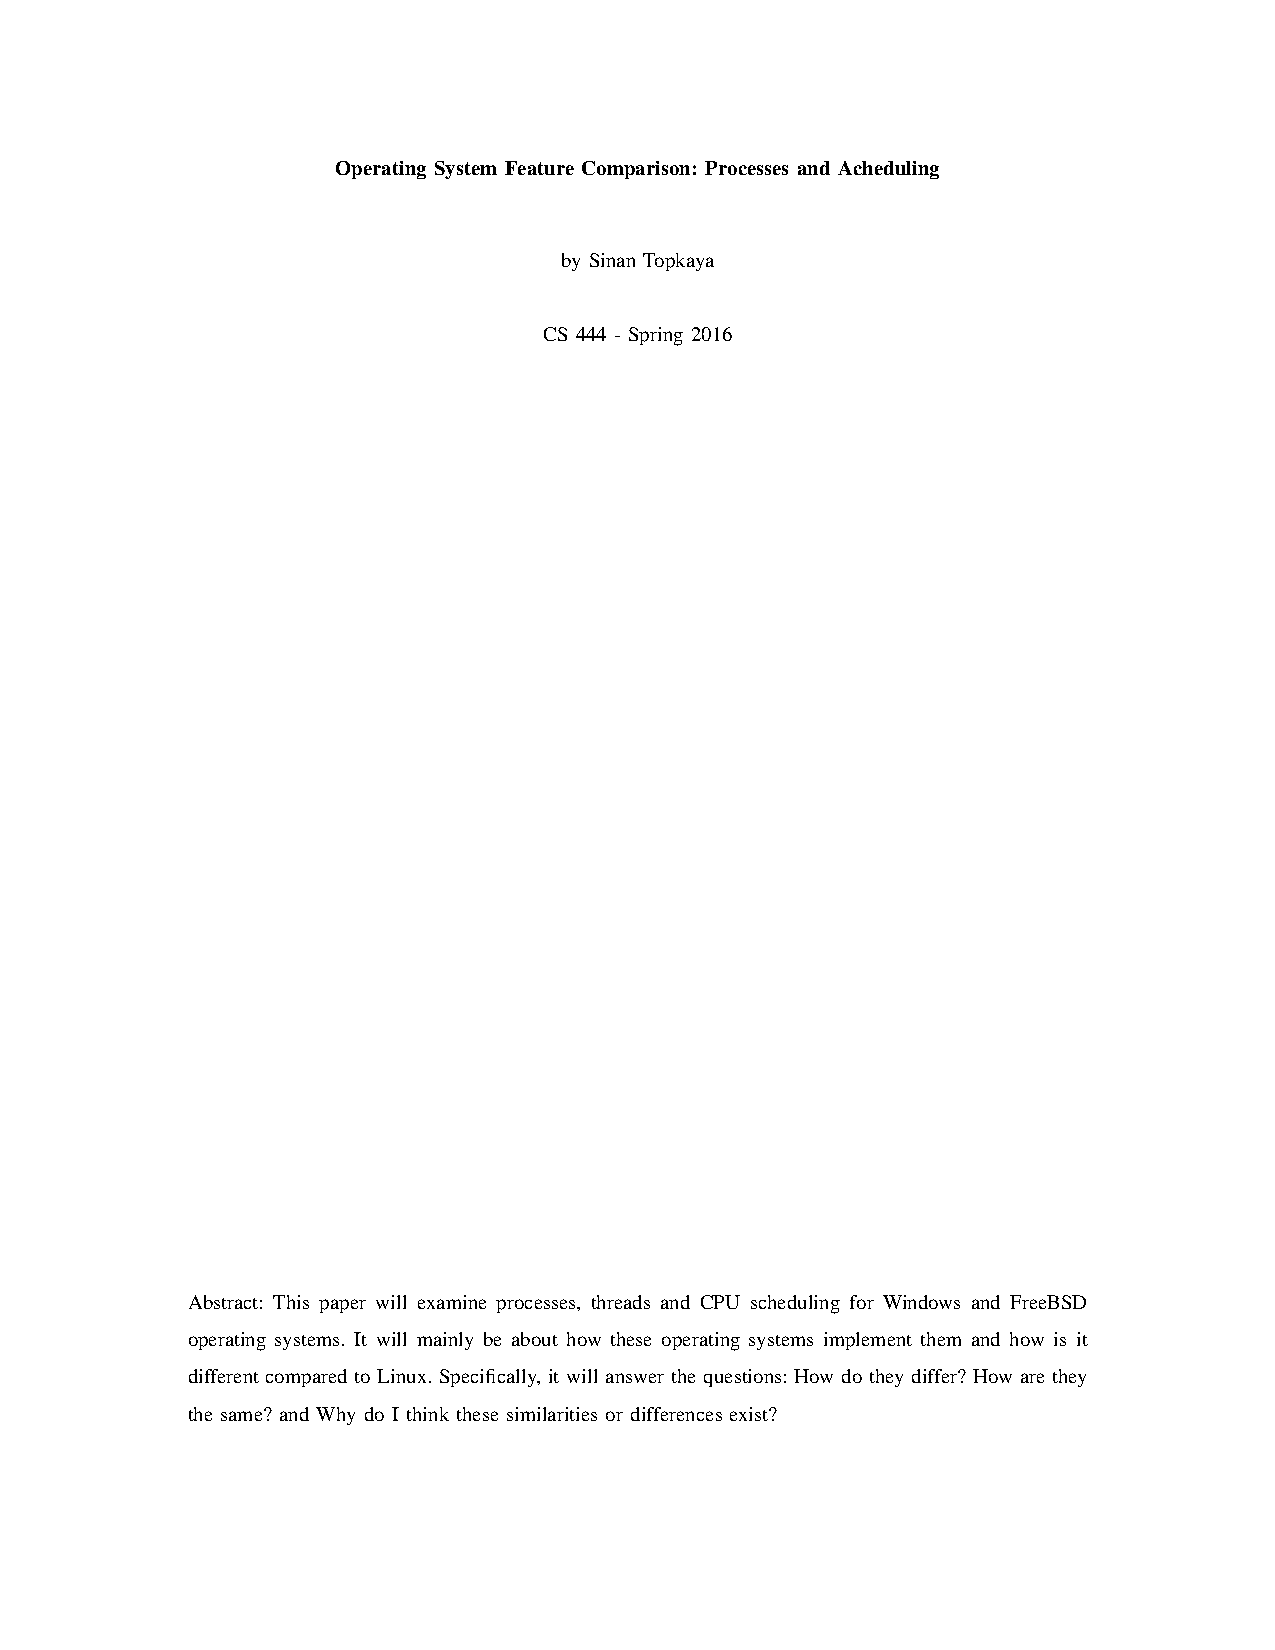
\includepdf[pages=-]{writing1.pdf}


\bibliographystyle{IEEEtran}
\bibliography{bibfile.bib}

\end{document}



